\documentclass[10pt, a4paper]{article}
\usepackage{amsmath,amssymb}
\usepackage{lmodern}
\usepackage[T1]{fontenc}
\usepackage[utf8]{inputenc}
\usepackage{textcomp}

\usepackage{hyperref}
\hypersetup{
  pdftitle={dyngen: a multi-modal simulator for spearheading new single-cell omics analyses},
  pdfauthor={Robrecht Cannoodt; Wouter Saelens; Louise Deconinck; Yvan Saeys},
  hidelinks}
\usepackage[margin=1in]{geometry}
\usepackage{graphicx}



\title{dyngen: a multi-modal simulator for spearheading new single-cell omics analyses}
\author{Robrecht Cannoodt\textsuperscript{$\dagger{}$,1,2,3} \and Wouter Saelens\textsuperscript{$\dagger{}$,1,2,4} \and Louise Deconinck\textsuperscript{1,2} \and Yvan Saeys\textsuperscript{1,2,*}}
\date{12 May 2021}

\begin{document}
\maketitle

\textsuperscript{1} Data Mining and Modelling for Biomedicine group, VIB
Center for Inflammation Research, Ghent, Belgium

\textsuperscript{2} Department of Applied Mathematics, Computer Science,
and Statistics, Ghent University, Ghent, Belgium

\textsuperscript{3} Data Intuitive, Lebbeke, Belgium

\textsuperscript{4} Institute of Bioengineering, School of Life
Sciences, École Polytechnique Fédérale de Lausanne (EPFL), Lausanne,
Switzerland

\textsuperscript{$\dagger{}$} These authors contributed equally to this work.

\textsuperscript{*} Correspondence: \texttt{yvan.saeys@ugent.be}

\section{Abstract}\label{abstract}

We present dyngen, a novel, multi-modal simulation engine for studying
dynamic cellular processes at single-cell resolution. dyngen is more
flexible than current single-cell simulation engines, and allows better
method development and benchmarking, thereby stimulating development and
testing of novel computational methods. We demonstrate its potential for
spearheading novel computational methods on three novel applications:
aligning cell developmental trajectories, cell-specific regulatory
network inference and estimation of RNA velocity.

\section{Introduction}\label{introduction}

Single-cell simulation engines are becoming increasingly important for
testing and benchmarking computational methods, a pressing need in the
widely expanding field of single-cell biology. Complementary to real
biological data, synthetic data provides a valuable alternative where
the actual ground truth is completely known and thus can be compared to,
in order to make quantitative evaluations of computational methods that
aim to reconstruct this ground truth
\cite{zappia_splattersimulationsinglecell_2017}. In addition,
simulation engines are more flexible when it comes to stress-testing
computational methods, for example by varying the parameters of the
simulation, such as the amount of noise, samples, and cells measured,
allowing benchmarking of methods over a wide range of possible
scenarios. In this way, they can even guide the design of real
biological experiments, finding out the best conditions to be used as
input for subsequent computational pipelines.

Another, more experimental use of simulation engines is their important
role in spearheading the development of novel computational methods,
possibly even before real data is available. In this way, simulation
engines can be used to assess the value of novel experimental protocols
or treatments. Simulation engines are also increasingly important when
it comes to finding alternatives to animal models, for example for drug
testing and precision medicine. In such scenarios, cellular simulations
can act as digital twins, offering unlimited experimentation \emph{in
silico} \cite{bjornsson_digitaltwinspersonalize_2019}.

Simulating realistic data requires that the underlying biology is
recapitulated as best as possible, and in the case of transcriptomics
data this typically involves modelling the underlying gene regulatory
networks. Simulators of ``bulk'' microarray or RNA-sequencing profiles
simulate biological processes (e.g.~transcription, translation) by
translating a database of known regulatory interactions into a set of
ordinary differential equations (ODE)
\cite{roy_systemgeneratingtranscription_2008,hache_gengesystematicgeneration_2009,schaffter_genenetweaversilicobenchmark_2011,vandenbulcke_syntrengeneratorsynthetic_2006}.
These methods have been instrumental in performing benchmarking studies
\cite{prill_rigorousassessmentsystems_2010,marbach_revealingstrengthsweaknesses_2010,marbach_wisdomcrowdsrobust_2012}.
However, the advent of single-cell omics introduced several new types of
analyses (e.g.~trajectory inference, RNA velocity, cell-specific network
inference) which exploit the higher resolution of single-cell versus
bulk omics \cite{luecken_currentbestpractices_2019}. In addition,
the data characteristics of single-cell omics are vastly different from
bulk omics, typically having much lower library sizes and a higher
dropout rate, but also a high number of profiles
\cite{vallejos_normalizingsinglecellrna_2017}. The low library
sizes, in particular, are problematic as ODEs are ill-suited for
performing low-molecule simulations
\cite{gillespie_exactstochasticsimulation_1977}. This necessitates
the development of new single-cell simulators.

To this end, single-cell omics simulators emulate the technical
procedures from single-cell omics protocols. Simulators such as Splatter
\cite{zappia_splattersimulationsinglecell_2017}, powsimR
\cite{vieth_powsimrpoweranalysis_2017}, PROSSTT
\cite{papadopoulos_prossttprobabilisticsimulation_2019} and SymSim
\cite{zhang_simulatingmultiplefaceted_2019}) have already been
widely used to compare single-cell methods
\cite{street_slingshotcelllineage_2018,parra_reconstructingcomplexlineage_2019,lummertzdarocha_reconstructioncomplexsinglecell_2018,lin_scclassifysamplesize_2020}
and perform independent benchmarks
\cite{duo_systematicperformanceevaluation_2018,saelens_comparisonsinglecelltrajectory_2019,soneson_biasrobustnessscalability_2018}.
However, by focusing more on simulating the single-cell omics protocol
(e.g.~RNA capture, amplification, sequencing) and less on the underlying
biology (e.g.~transcription, splicing, translation), their applicability
and reusability is limited towards the specific application for which
they were designed (e.g.~benchmarking clustering or differential
expression methods), and extending these tools to include additional
modalities or experimental conditions is challenging.

We introduce dyngen, a method for simulating cellular dynamics at a
single-cell, single-transcript resolution (Figure~\ref{fig:overview}).
This problem is tackled in three fully-configurable main steps. First,
biological processes are mimicked by translating a gene regulatory
network into a set of reactions (regulation, transcription, splicing,
translation). Second, individual cells are simulated using Gillespie's
stochastic simulation algorithm
\cite{gillespie_exactstochasticsimulation_1977}, which is designed
to work well in low-molecule simulations. Finally, real reference
datasets are used to emulate single-cell omics profiling protocols.

Throughout a simulation, dyngen tracks many layers of information,
including the abundance of any molecule in the cell, the progression of
the cell along a dynamic process, and the activation strength of
individual regulatory interactions. In addition, dyngen can simulate a
large variety of dynamic processes (e.g.~cyclic, branching,
disconnected) as well as a broad range of experimental conditions
(e.g.~batch effects and time-series, perturbation and single-cell
knockdown experiments). For these reasons, dyngen can cater to a wide
range of benchmarking applications, including trajectory inference,
trajectory alignment, and trajectory differential expression
(Supplementary Table~1).

\begin{figure}[htbp]
    \centering
    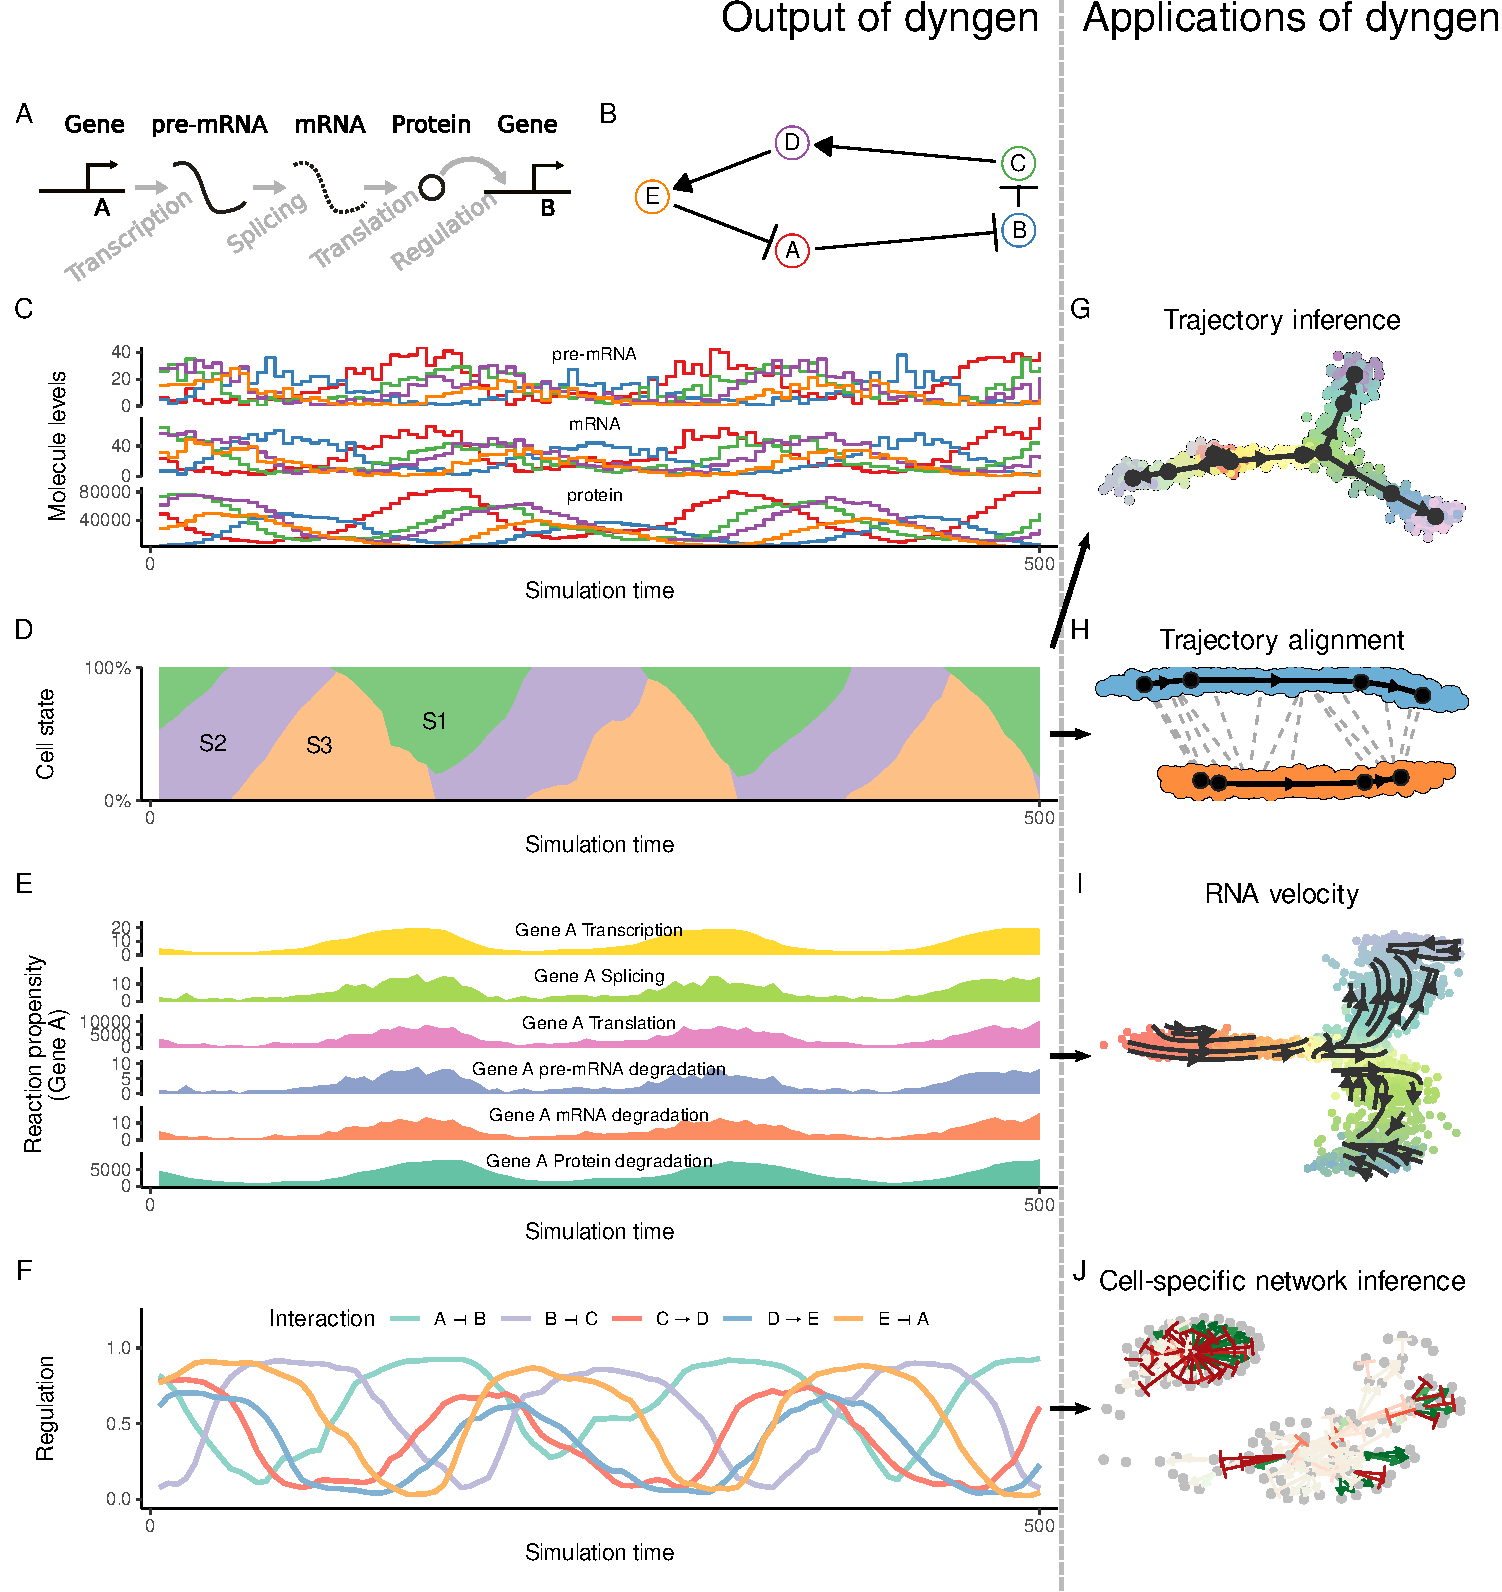
\includegraphics[width=\linewidth]{figure_1.pdf}
    \caption{
      \textbf{Showcase of dyngen functionality.}
      \textbf{A:} Changes in abundance levels are driven strictly by gene regulatory reactions.
      \textbf{B:} The input Gene Regulatory Network (GRN) is defined such that it models a dynamic process of interest.
      \textbf{C:} The reactions define how abundance levels of molecules change at any particular time point.
      \textbf{D:} Firing many reactions can significantly alter the cellular state over time.
      \textbf{E:} dyngen keeps track of the likelihood of a reaction firing during small intervals of time, called the propensity, as well as the actual number of firings.
      \textbf{F:} Similarly, dyngen can also keep track of the regulatory activity of every interaction.
      \textbf{G:} A benchmark of trajectory inference methods has already been performed using the cell state ground-truth \cite{saelens_comparisonsinglecelltrajectory_2019}.
      \textbf{H:} The cell state ground-truth enables evaluating trajectory alignment methods.
      \textbf{I:} The reaction propensity ground-truth enables evaluating RNA velocity methods.
      \textbf{J:} The cellwise regulatory network ground-truth enables evaluating cell-specific gene regulatory network inference methods.
    }
    \label{fig:overview}
\end{figure}

\section{Results}\label{results}

We demonstrate dyngen's broad applicability by evaluating three novel
types of computational approaches for which no simulation engines exist
yet: cell-specific network inference, trajectory alignment and RNA
velocity (Figure~\ref{fig:applications}). We emphasize that our main aim
here is to illustrate the potential of dyngen for these evaluations,
rather than performing large-scale benchmarking, which would require
assessing many more quantitative and qualitative aspects of each method
\cite{weber_essentialguidelinescomputational_2019}.

\begin{figure}[htbp]
    \centering
    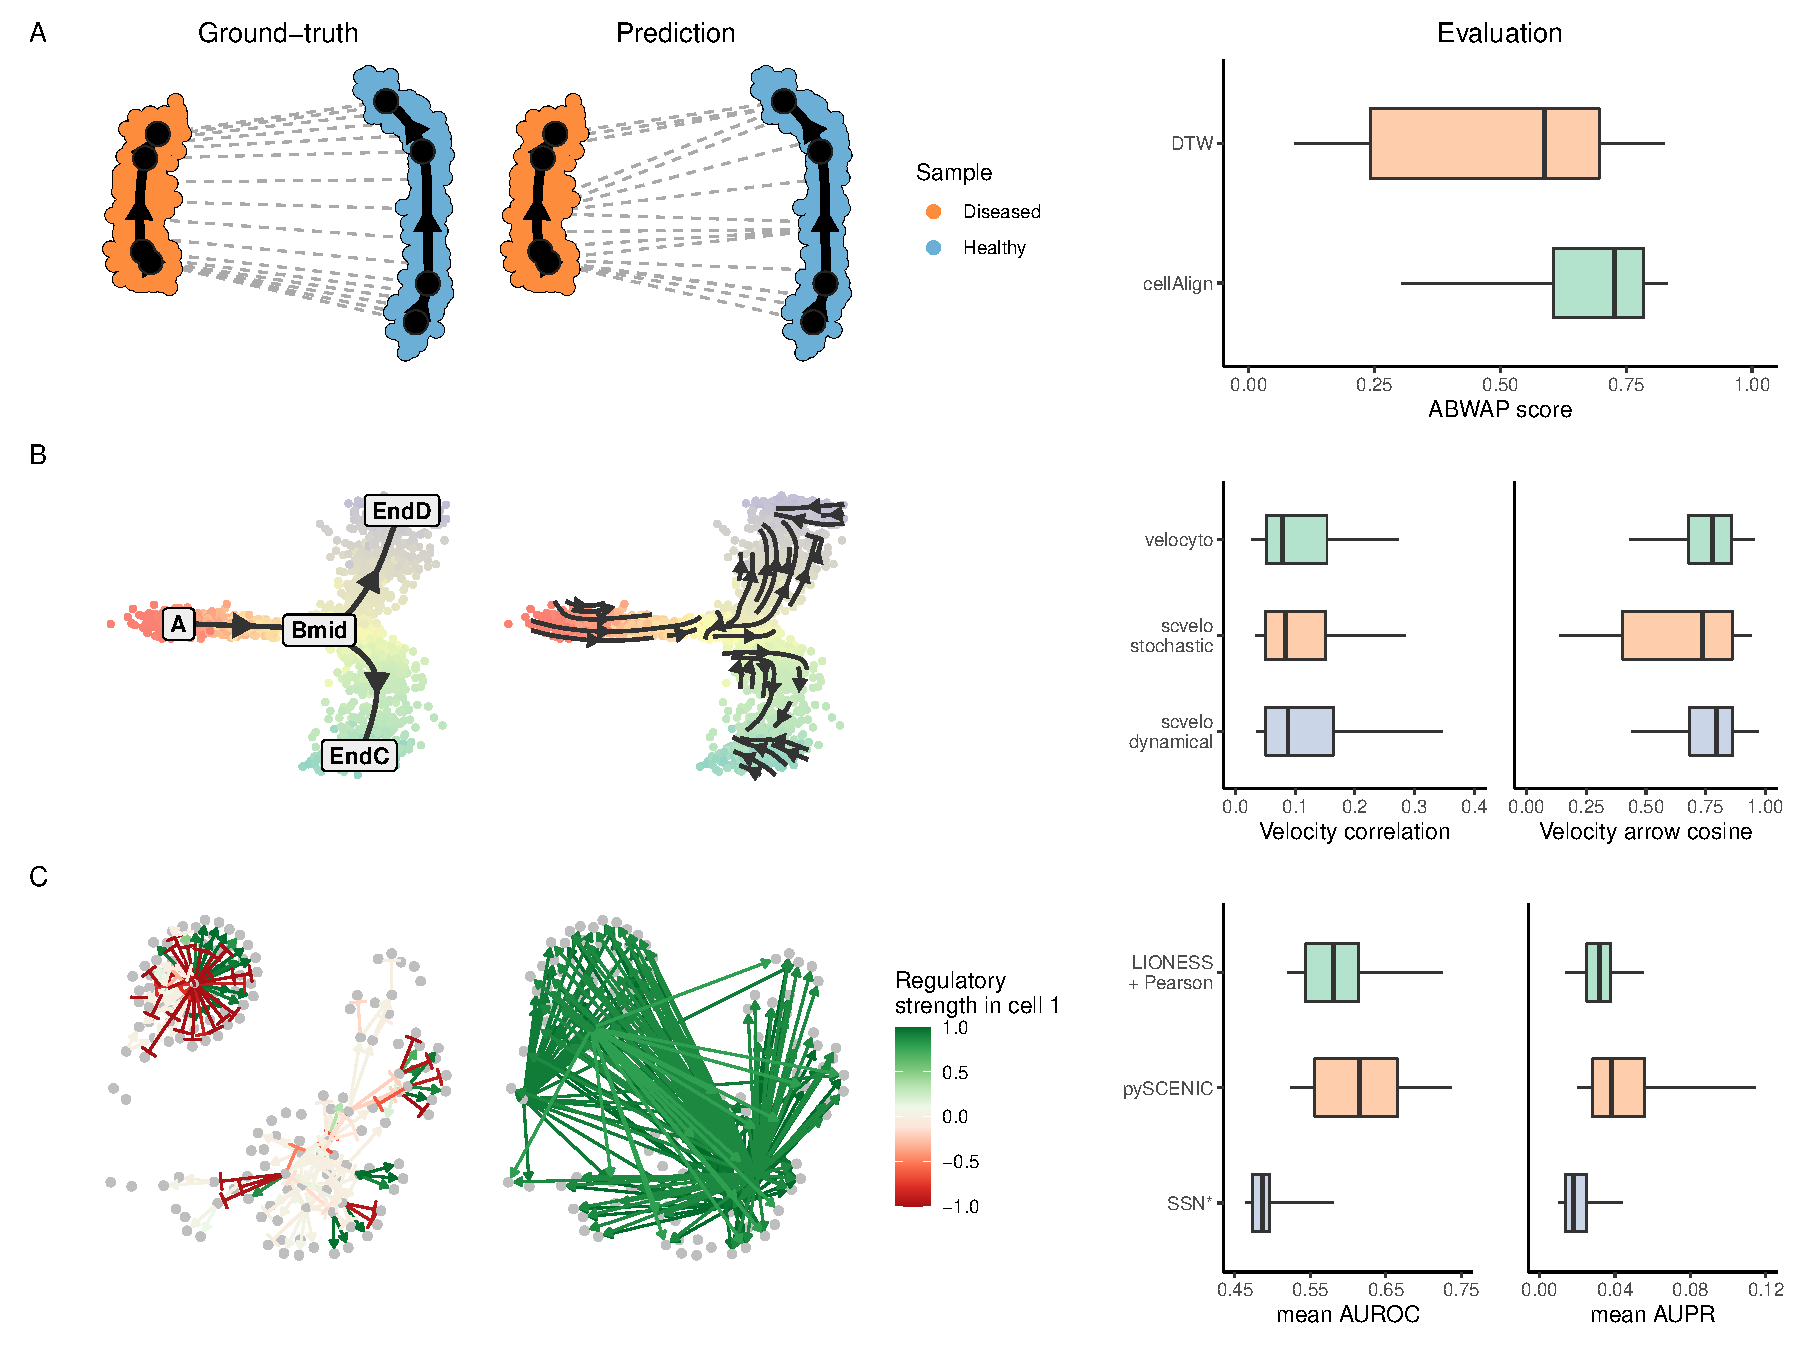
\includegraphics[width=\linewidth]{figure_2.pdf}
    \caption{
      \textbf{dyngen provides ground-truth data for a variety of applications (left), which can be used to quantitatively evaluate methods (right).} Box plots denote the $Q_0$ to $Q_4$ quartile values.
      \textbf{A:} Trajectory alignment aligns two trajectories between samples. We evaluate dynamic time warping (DTW) and cellAlign when aligning two linear trajectories with different kinetic parameters based on the area differences between the worst possible alignment and the predicted alignment (Area Between Worst And Prediction, or ABWAP). 
      \textbf{B:} RNA velocity calculates for each cell the direction in which the expression of each gene is moving. We evaluated scVelo and velocyto by comparing these vectors with the known velocity vector (velocity correlation) and with the known direction of the cellular trajectory in a dimensionality reduction (velocity arrow cosine).
      \textbf{C:} Cell-specific network inference (CSNI) predicts the regulatory network of every individual cell. We evaluate each cell-specific regulatory network with typical metrics for network inference: the Area Under the Receiver Operating Characteristics-curve (AUROC) and Area Under the Precision Recall-curve (AUPR). We evaluate three CSNI methods by computing the mean AUROC and AUPR across all cells.
    }
    \label{fig:applications}
\end{figure}

Use-case ``trajectory alignment''. Trajectory alignment methods align
trajectories from different samples and allow studying the differences
between the different trajectories. For example, by comparing the
transcriptomic profiles of cells from a diseased patient to a healthy
control, it might be possible to detect transcriptomics differences
(differential expression) of particular cells along a developmental
process, or to detect an early stop of the trajectory of the diseased
patient. Currently, trajectory alignment is limited to aligning linear
trajectories, though other topologies of a trajectory could be aligned
as well. Dynamic Time Warping (DTW)
\cite{giorgino_computingvisualizingdynamic_2009} is a method
designed for aligning temporal sequences for speech recognition but has
since been used to compare gene expression kinetics from many different
biological processes
\cite{cacchiarelli_aligningsinglecelldevelopmental_2018,kanton_organoidsinglecellgenomic_2019,mcfaline-figueroa_pooledsinglecellgenetic_2019,alpert_alignmentsinglecelltrajectories_2018}.
cellAlign \cite{alpert_alignmentsinglecelltrajectories_2018} uses
DTW to perform trajectory alignment, but also includes interpolation and
scaling of the single cell data as a preprocessing step. We evaluate the
performance of DTW and cellAlign by simulating 40 datasets, each
containing two linear trajectories generated with the same gene
regulatory network but with slightly different simulation kinetics. We
assess the accuracy of the obtained alignments by comparing the
generated alignment path with the worst possible alignment that could be
performed (Supplementary Fig. ~1D), named the Area Between Worst And
Prediction (ABWAP) score. Overall, cellAlign performs significantly
better than DTW (Supplementary Fig.~1), which is likely due to the
interpolation and scaling steps provided by cellAlign, reducing noise in
the data and improving the comparability of the trajectories. Note that,
in this comparison, only linear trajectory alignment is performed. While
dyngen can generate non-linear trajectories (e.g.~cyclic or branching),
both aligning non-linear trajectories and constructing a quantitative
accuracy metric for non-linear trajectory alignment is not trivial and
an avenue for future work.

Use-case ``RNA velocity''. RNA velocity methods use the relative ratio
between pre-mRNA and mature mRNA reads to predict the rate of
increase/decrease of RNA molecule abundance, as this can be used to
predict the directionality of single cell differentiation in
trajectories
\cite{zeisel_coupledpremrnamrna_2011,lamanno_rnavelocitysingle_2018}.
Already two algorithms are currently available for estimating the RNA
velocity vector from spliced and unspliced counts: velocyto
\cite{lamanno_rnavelocitysingle_2018} and scvelo
\cite{bergen_generalizingrnavelocity_2020}. Yet, to date, no
quantitative assessment of their accuracy has been performed, mainly due
to the difficulty in obtaining real ground-truth data to do so. In
contrast, the ground-truth RNA velocity can be easily extracted from a
dyngen simulation, as it is possible to store the rate at which mRNA
molecules are being transcribed and degraded at any particular point in
time. We executed velocyto and scvelo (with 2 different parameter
settings, stochastic and dynamical) on 42 datasets with a variety of
backbones (including linear, bifurcating, cyclic, disconnected). We
evaluated the predictions using two metrics (Supplementary Fig.~2), one
which directly compares the predicted RNA velocity of each gene with the
ground-truth RNA velocity (called the ``velocity correlation''), and one
which compares the direction of the ground-truth trajectory embedded in
a dimensionality reduction with the average RNA velocity of cells in
that neighbourhood (called the ``velocity arrow cosine''). While both
velocyto and scvelo obtained high scores for the velocity arrow cosine
metric (overall 25th percentile = 0.606), the velocity correlation is
rather low (overall 75th percentile = 0.156). This means that predicting
the RNA velocity (i.e.~transcription rate minus the decay rate) for
particular individual genes can be challenging, but the combined
information is very informative in determining the directionality of
cell progression in the trajectory. In terms of velocity correlation, no
method performed significantly better than the other, whereas ``scvelo
stochastic'' performed slightly worse than ``scvelo dynamical'' and
velocyto in terms of velocity arrow cosine score. Note that, given that
some genes are more informative in determining the overall
directionality of cell progression, performing a feature selection
before computing the embedded dimensionality reduction might result in
significantly improved velocity arrow cosine scores.

Use-case ``Cell-specific network inference'' (CSNI). CSNI methods
predict not only which transcription factors regulate which target
genes, but also aim to identify how active each interaction is in each
of the cells, since interactions can be turned off and on depending on
the cellular state. While a few pioneering CSNI approaches have already
been developed
\cite{aibar_scenicsinglecellregulatory_2017,kuijjer_estimatingsamplespecificregulatory_2019,liu_personalizedcharacterizationdiseases_2016},
a quantitative assessment of their performance is until now lacking.
This is not surprising, as neither real nor in silico datasets of
cell-specific or even cell-type-specific interactions exist that are
large enough so that it can be used as a ground-truth for evaluating
CSNI methods. Extracting the ground-truth dynamic network in dyngen is
straightforward though, given that we can calculate how target gene
expression would change without the regulator being present. We used
this ground-truth to compare the performance of three CSNI methods
(Supplementary Fig.~3): LIONESS
\cite{kuijjer_estimatingsamplespecificregulatory_2019}, SSN
\cite{liu_personalizedcharacterizationdiseases_2016} and SCENIC
\cite{aibar_scenicsinglecellregulatory_2017}. For each dataset, we
computed the mean AUROC and AUPR scores of the individual cells.
Comparing the mean AUROC and AUPR showed that pySCENIC significantly
outperforms both LIONESS and SSN, and in turn that LIONESS significantly
outperforms SSN. The poor performance of SSN is expected, as its
methodology for predicting a cell-specific is simply computing the
difference in Pearson correlation values applied to the whole dataset
and the whole dataset minus one sample. This strategy performs poorly in
large datasets where cell correlations are high, as the removal of one
cell will not yield large differences in correlation values and will
result in mostly noise. Overall, pySCENIC almost always performs better
than LIONESS, except for a few datasets where LIONESS does manage to
obtain a higher AUROC score. However, by using a different internal
network inference (e.g.~GENIE3
\cite{huynh-thu_inferringregulatorynetworks_2010} or pySCENIC's
GRNBoost2 \cite{moerman_grnboost2arboretoefficient_2019}) could
significantly increase the performance obtained by LIONESS.

\section{Discussion}\label{discussion}

dyngen's single-cell simulations can be used to evaluate common
single-cell omics computational methods such as clustering, batch
correction, trajectory inference, and network inference. However, the
framework is flexible enough to be adaptable to a broad range of
applications, including methods that integrate clustering, network
inference, and trajectory inference. In this respect, dyngen may promote
the development of new tools in the single-cell field similarly as other
simulators have done in the past
\cite{schaffter_genenetweaversilicobenchmark_2011,ewing_combiningtumorgenome_2015}.
Additionally, one could anticipate technological developments in
single-cell multi-omics. In this way, dyngen allows designing and
evaluating the performance and robustness of new types of computational
analyses before experimental data becomes available, comparing which
experimental protocol is the most cost-effective in producing
qualitative and robust results in downstream analysis. One major
assumption of dyngen is that cells are assumed to be well-mixed and
independent from each other. Subdividing a cell into multiple 2D or 3D
subvolumes or allowing cells to exchange molecules, respectively, could
pave the way to better study key cellular processes such as cell
division, intercellular communication, and migration
\cite{smith_spatialstochasticintracellular_2019}.

\newpage

\section{Methods}\label{sec:dyngen-methods}

The workflow to generate \emph{in silico} single-cell data consists of
six main steps (Supplementary Fig~4).

\subsection{Defining the module network}\label{sec:dyngen-modules}

One of the main processes involved in cellular dynamic processes is gene
regulation, where regulatory cascades and feedback loops lead to
progressive changes in expression and decision making. The exact way a
cell chooses a certain path during its differentiation is still an
active research field, although certain models have already emerged and
been tested \emph{in vivo}. One driver of bifurcation is mutual
antagonism, where two genes strongly repress each other
\cite{rekhtman_directinteractionhematopoietic_1999,xu_regulationbifurcatingcell_2015},
forcing one of the two to become inactive
\cite{graf_forcingcellschange_2009}. Such mutual antagonism can be
modelled and simulated
\cite{wang_quantifyingwaddingtonlandscape_2011,ferrell_bistabilitybifurcationswaddington_2012}.
Although the two-gene model is simple and elegant, the reality is
frequently more complex, with multiple genes (grouped into modules)
repressing each other \cite{yosef_dynamicregulatorynetwork_2013}.

To start a dyngen simulation, the user needs to define a module network.
The module network describes how sets of genes regulate each other and
is what mainly determines which dynamic processes occur within the
simulated cells.

A module network consists of modules connected together by regulatory
interactions, which can be either up- or down-regulating. A module may
have basal expression, which means genes in this module will be
transcribed without the presence of transcription factor molecules. A
module marked as ``active during the burn phase'' means that this module
will be allowed to generate expression of its genes during an initial
warm-up phase. At the end of the
dyngen process, cells will not be sampled from the burn phase
simulations. Interactions between modules have a strength (which is a
positive integer) and an effect (+1 for upregulating, -1 for
downregulating).

Several examples of module networks are given in Supplementary Fig.~5. A
simple chain of modules (where one module upregulates the next) results
in a \emph{linear} process. By having the last module repress the first
module, the process becomes \emph{cyclic}. Two modules repressing each
other is the basis of a \emph{bifurcating} process, though several
chains of modules have to be attached in order to achieve progression
before and after the bifurcation process. Finally, a \emph{converging}
process has a bifurcation occurring during the burn phase, after which
any differences in module regulation is removed.

Note that these examples represent the bare minimum in terms of the
number of modules used. Using longer chains of modules is typically
desired. In addition, the fate decisions made in this example of a
bifurcation is reversible, meaning cells can be reprogrammed to go down
a different differentiation path. If this effect is undesirable, more
safeguards need to be put in place to prevent reprogramming from
occurring.

\subsection{Generating the gene regulatory network}\label{sec:dyngen-grn}

The GRN is generated based on the given module network in four main
steps (Supplementary Fig.~6).

Step 1, sampling the transcription factors (TF). The TFs are the main
drivers of the molecular changes in the simulation. The user provides a
backbone and the number of TFs to generate. Each TF is assigned to a
module such that each module has at least \(x\) parameters (default
\(x=1\)). A TF inherits the `burn' and `basal expression' from the
module it belongs to.

Step 2, generating the TF interactions. Let each TF be regulated
according to the interactions in the backbone. These interactions
inherit the effect, strength, and independence parameters from the
interactions in the backbone. A TF can only be regulated by other TFs or
itself.

Step 3, sampling the target subnetwork. A user-defined number of target
genes are added to the GRN. Target genes are regulated by a TF or
another target gene, but are always downstream of at least one TF. To
sample the interactions between target genes, one of the many FANTOM5
\cite{lizio_gatewaysfantom5promoter_2015} GRNs is sampled. The
currently existing TFs are mapped to regulators in the FANTOM5 GRN. The
targets are drawn from the FANTOM5 GRN weighted by their page rank
value, to create an induced GRN. For each target, at most \(x\)
regulators are sampled from the induced FANTOM5 GRN (default \(x=5\)).
The interactions connecting a target gene and its regulators are added
to the GRN.

Step 4, sampling the housekeeping subnetwork. Housekeeping genes are
completely separate from any TFs or target genes. A user-defined set of
housekeeping genes is also sampled from the FANTOM5 GRN. The
interactions of the FANTOM5 GRN are first subsampled such that the
maximum in-degree of each gene is \(x\) (default \(x=5\)). A random gene
is sampled and a breadth-first-search is performed to sample the desired
number of housekeeping genes.

\subsection{Convert gene regulatory network to a set of reactions}\label{sec:dyngen-reactions}

\newcommand{\x}[1]{\text{x}_{#1}}
\newcommand{\y}[1]{\text{y}_{#1}}
\newcommand{\z}[1]{\text{z}_{#1}}

\newcommand{\rs}[1]{\text{R}_{#1}}
\newcommand{\rp}[1]{\text{R}^+_{#1}}
\newcommand{\rn}[1]{\text{R}^-_{#1}}

\newcommand{\xpr}[1]{\text{xpr}_{#1}}
\newcommand{\xhl}[1]{\text{xhl}_{#1}}
\newcommand{\ysr}[1]{\text{ysr}_{#1}}
\newcommand{\yhl}[1]{\text{yhl}_{#1}}
\newcommand{\ydr}[1]{\text{ydr}_{#1}}
\newcommand{\zpr}[1]{\text{zpr}_{#1}}
\newcommand{\zhl}[1]{\text{zhl}_{#1}}
\newcommand{\zdr}[1]{\text{zdr}_{#1}}

\newcommand{\str}[1]{\text{str}_{#1}}
\newcommand{\hill}[1]{\text{hill}_{#1}}
\newcommand{\ind}[1]{\text{ind}_{#1}}
\newcommand{\dis}[1]{\text{dis}_{#1}}
\newcommand{\buf}[1]{\text{bind}_{#1}}
\newcommand{\ba}[1]{\text{bas}_{#1}}

Simulating a cell's GRN makes use of a stochastic framework which tracks
the abundance levels of molecules over time in a discrete quantity. For
every gene \(G\), the abundance levels of three molecules are tracked,
namely of corresponding pre-mRNAs, mature mRNAs and proteins, which are
represented by the terms \(\text{x}_{G}\), \(\text{y}_{G}\) and
\(\text{z}_{G}\) respectively. The GRN defines how a reaction affects
the abundance levels of molecules and how likely it will occur. Gibson
and Bruck \cite{gibson_probabilisticmodelprokaryotic_2000} provide a
good introduction to modelling gene regulation with stochastic
frameworks, on which many of the concepts below are based.

For every gene in the GRN a set of reactions are defined, namely
transcription, splicing, translation, and degradation. Each reaction
consists of a propensity function -- a formula \(f(.)\) to calculate the
probability \(f(.) \times \text{d}t\) of it occurring during a time
interval \(\text{d}t\) -- and the effect -- how it will affect the
current state if triggered.

The effects of each reaction mimic the respective biological processes
(Supplementary Table~2, middle). Transcription of gene \(G\) results in
the creation of a single pre-mRNA molecule \(\text{x}_{G}\). Splicing
turns one pre-mRNA \(\text{x}_{G}\) into a mature mRNA \(\text{x}_{G}\).
Translation uses a mature mRNA \(\text{y}_{G}\) to produce a protein
\(\text{z}_{G}\). Pre-mRNA, mRNA and protein degradation results in the
removal of a \(\text{x}_{G}\), \(\text{y}_{G}\), and \(\text{z}_{G}\)
molecule, respectively.

The propensity of all reactions except transcription are all linear
functions (Supplementary Table~2, right) of the abundance level of some
molecule multiplied by a per-gene constant (Supplementary Table~3). The
propensity of transcription of a gene \(G\) depends on the abundance
levels of its TFs. The per-gene and per-interaction constants are based
on the median reported production-rates and half-lives of molecules
measured of 5000 mammalian genes
\cite{schwanhausser_globalquantificationmammalian_2011}, except that
the transcription rate has been amplified by a factor of 10.

\newcommand{\proptran}{f}
\newcommand{\ai}[2]{$S_{#1} = S_{#2b}$}
\newcommand{\zk}[1]{\frac{y_#1}{k_#1}^{c_#1}}
\newcommand{\wi}[1]{\nu_#1}

The propensity of the transcription of a gene \(G\) is inspired by
thermodynamic models of gene regulation
\cite{schilstra_biologicgeneexpression_2008}, in which the promoter
of \(G\) can be bound or unbound by a set of \(N\) transcription factors
\(H_i\). Let \(f(\text{z}_{1}, \text{z}_{2}, \ldots, \text{z}_{N})\)
denote the propensity function of \(G\), in function of the abundance
levels of the transcription factors. The following subsections explain
and define the propensity function when \(N=1\), \(N=2\), and finally
for an arbitrary \(N\).

\subsubsection{\texorpdfstring{Propensity of transcription when \(N=1\)}{Propensity of transcription when N=1}}\label{propensity-of-transcription-when-n1}

In the simplest case when \(N=1\), the promoter can be in one of two
states. In state \(S_0\), the promoter is not bound by any transcription
factors, and in state \(S_1\) the promoter is bound by \(H_1\). Each
state \(S_j\) is linked with a relative activation \(\alpha_j\), a
number between 0 and 1 representing the activity of the promoter at this
particular state. The propensity function is thus equal to the expected
value of the activity of the promoter multiplied by the pre-mRNA
production rate of \(G\).

\begin{align}
  f(y_1, y_2, \ldots, y_N) & = \text{xpr} \cdot \sum_{j = 0}^{2^N - 1} \alpha_j \cdot P(S_j) \label{eqn:activ0} 
\end{align}

For \(N=1\), \(P(S_1)\) is equal to the Hill equation, where \(k_i\)
represents the concentration of \(H_i\) at half-occupation and \(n_i\)
represents the Hill coefficient. Typically, \(n_i\) is between
{[}1,10{]}

\begin{align}
  P(S_1) & = \frac{y_1^{n_1}}{k_1^{n_1} + y_1^{n_1}} \\
             & = \frac{(y_1/k_1)^{n_1}}{1 + (y_1/k_1)^{n_1}}
\end{align}

The Hill equation can be simplified by letting
\(\nu_i = \left(\frac{y_i}{k_i}\right)^{n_i}\).

\begin{align}
P(S_1) & = \frac{\nu_1}{1 + \nu_1} \label{eqn:hillsimp}
\end{align}

Since \(P(S_0) = 1 - P(S_1)\), the activation function is formulated and
simplified as follows.

\begin{align}
f(y_1) & = \text{xpr} \cdot \left(\alpha_0 \cdot P(S_0) + \alpha_1 \cdot P(S_1)\right) \\
           & = \text{xpr} \cdot \left(\alpha_0 \cdot \frac{1}{1 + \nu_1} + \alpha_1 \cdot \frac{\nu_1}{1 + \nu_1}\right) \\
           & = \text{xpr} \cdot \frac{\alpha_0 + \alpha_1 \cdot \nu_1}{1 + \nu_1} \\
\end{align}

\subsubsection{\texorpdfstring{Propensity of transcription when \(N=2\)}{Propensity of transcription when N=2}}\label{propensity-of-transcription-when-n2}

When \(N=2\), there are four states \(S_j\). The relative activations
\(\alpha_j\) can be defined such that \(H_1\) and \(H_2\) are
independent (additive) or synergistic (multiplicative). In order to
define the propensity of transcription \(f(.)\), the Hill equation
\(P(S_j)\) is extended for two transcription factors.

Let \(w_j\) be the numerator of \(P(S_j)\), defined as the product of
all transcription factors bound in that state:

\begin{align}
w_0 & = 1 \\
w_1 & = \nu_1 \\
w_2 & = \nu_2 \\
w_3 & = \nu_1 \cdot \nu_2
\end{align}

The denominator of \(P(S_j)\) is then equal to the sum of all \(w_j\).
The probability of state \(S_j\) is thus defined as:

\begin{align}
    P(S_j) & = \frac{w_j}{\sum_{j=0}^{j < 2^N} w_j} \\
               & = \frac{w_j}{1 + \nu_1 + \nu_2 + \nu_1 \cdot \nu_2} \\
               & = \frac{w_j}{\prod_{i=1}^{i \leq N} (\nu_i + 1)}
\end{align}

Substituting \(P(S_j)\) and \(w_j\) into \(f(.)\) results in the
following equation:

\begin{align}
f(y_1, y_2) & = \text{xpr} \cdot \sum_{j = 0}^{2^N - 1} \alpha_j \cdot P(S_j) \\
 & = \text{xpr} \cdot \frac{\sum_{j = 0}^{2^N - 1} \alpha_j \cdot w_j}{\prod_{i=1}^{i \leq N} (\nu_i + 1)} \\
 & = \text{xpr} \cdot \frac{\alpha_0 + \alpha_1 \cdot \nu_1 + \alpha_2 \cdot \nu_2 + \alpha_3 \cdot \nu_1 \cdot \nu_2}{(\nu_1 + 1) \cdot (\nu_2 + 1)} \\
\end{align}

\subsubsection{\texorpdfstring{Propensity of transcription for an arbitrary \(N\)}{Propensity of transcription for an arbitrary N}}\label{propensity-of-transcription-for-an-arbitrary-n}

For an arbitrary \(N\), there are \(2^N\) states \(S_j\). The relative
activations \(\alpha_j\) can be defined such that \(H_1\) and \(H_2\)
are independent (additive) or synergistic (multiplicative). In order to
define the propensity of transcription \(f(.)\), the Hill equation
\(P(S_j)\) is extended for \(N\) transcription factors.

Let \(w_j\) be the numerator of \(P(S_j)\), defined as the product of
all transcription factors bound in that state:

\begin{align}
  w_j & = \prod_{i=1}^{i \leq N} (j \text{ mod } i) = 1 \text{ ? } \nu_i \text{ : } 1
\end{align}

The denominator of \(P(S_j)\) is then equal to the sum of all \(w_j\).
The probability of state \(S_j\) is thus defined as:

\begin{align}
P(S_j) & = \frac{w_j}{\sum_{j=0}^{j < 2^N} w_j} \\
& = \frac{w_j}{\prod_{i=1}^{i \leq N} (\nu_i + 1)}
\end{align}

Substituting \(P(S_j)\) into \(f(.)\) yields:

\begin{align}
f(y_1, y_2, \ldots, y_N) & = \text{xpr} \cdot \sum_{j = 0}^{2^N - 1} \alpha_j \cdot P(S_j) \\
& = \text{xpr} \cdot \frac{\sum_{j = 0}^{2^N - 1} \alpha_j \cdot w_j}{\prod_{i=1}^{i \leq N} (\nu_i + 1)} \label{eqn:prop2n}
\end{align}

\subsubsection{\texorpdfstring{Propensity of transcription for a large \(N\)}{Propensity of transcription for a large N}}\label{propensity-of-transcription-for-a-large-n}

For large values of \(N\), computing \(f(.)\) is practically infeasible
as it requires performing \(2^N\) summations. In order to greatly
simplify \(f(.)\), \(\alpha_j\) could be defined as 0 when one of the
regulators inhibits transcription and 1 otherwise.

\begin{equation}
\alpha_j = \begin{cases}
 0 & \text{ if } \exists i : j \text{ mod } i = 1 \text{ and } H_i \text{ represses } G \\
 1 & \text{otherwise}
\end{cases} \label{eqn:assalpha}
\end{equation}

Substituting equation \ref{eqn:assalpha} into equation \ref{eqn:prop2n}
and defining \(R = \{1, 2, \ldots, N\}\) and
\(R^+ = \{i | H_i \text{ activates } G\}\) yields the simplified
propensity function:

\begin{align}
f(y_1, y_2, \ldots, y_N) & = \text{xpr} \cdot \frac{\prod_{i \in R^+} (\nu_i + 1)}{\prod_{i \in R} (\nu_i + 1)}
\end{align}

\subsubsection{Independence, synergism and basal expression}\label{independence-synergism-and-basal-expression}

The definition of \(\alpha_j\) as in equation \ref{eqn:assalpha}
presents two main limitations. Firstly, since \(\alpha_0 = 1\), it is
impossible to tweak the propensity of transcription when no
transcription factors are bound. Secondly, it is not possible to tweak
the independence and synergism of multiple regulators.

Let \(\text{ba} \in [0,1]\) denote the basal expression strength \(G\)
(i.e.~how much will \(G\) be expressed when no transcription factors are
bound), and \(\text{sy} \in [0,1]\) denote the synergism of regulators
\(H_i\) of \(G\), the transcription propensity becomes:

\begin{align}
f(y_1, y_2, \ldots, y_N) & = \text{xpr} \cdot \frac{\text{ba} - \text{sy}^{|R^+|} + \prod_{i \in R^+} (\nu_i + \text{sy})}{\prod_{i \in R} (\nu_i + 1)}
\end{align}

\subsection{Simulate single cells}\label{dyngen-simcell}

dyngen uses Gillespie's stochastic simulation algorithm (SSA)
\cite{gillespie_exactstochasticsimulation_1977} to simulate dynamic
processes. An SSA simulation is an iterative process where at each
iteration one reaction is triggered.

Each reaction consists of its propensity -- a formula to calculate the
probability of the reaction occurring during an infinitesimal time
interval -- and the effect -- how it will affect the current state if
triggered. Each time a reaction is triggered, the simulation time is
incremented by
\(\tau = \frac{1}{\sum_j \textrm{prop}_j} \ln\left(\frac{1}{r}\right)\),
with \(r \in U(0, 1)\) and \(\textrm{prop}_j\) the propensity value of
the \(j\)th reaction for the current state of the simulation.

GillespieSSA2 is an optimised library for performing SSA simulations.
The propensity functions are compiled to C++ and SSA approximations can
be used which allow triggering many reactions simultaneously at each
iteration. The framework also allows storing the abundance levels of
molecules only after a specific interval has passed since the previous
census. By setting the census interval to 0, the whole simulation's
trajectory is retained but many of these time points will contain very
similar information. In addition to the abundance levels, also the
propensity values and the number of firings of each of the reactions at
each of the time steps can be retained.

\subsection{Simulate experiment}\label{sec:dyngen-experiment}

From the SSA simulation we obtain the abundance levels of all the
molecules at every state. We need to replicate technical effects
introduced by experimental protocols in order to obtain data that is
similar to real data. For this, the cells are sampled from the
simulations and molecules are sampled for each of the cells. Gene
capture rates and library sizes are empirically derived from real
datasets as to match real technical variation.

\subsubsection{Sample cells}\label{sample-cells}

In this step, \(N\) cells are sampled from the simulations. Two
approaches are implemented: sampling from an unsynchronised population
of single cells (snapshot) or sampling at multiple time points in a
synchronised population (time series).

\textbf{Snapshot} The backbone consists of several states linked
together by transition edges with length \(L_i\), to which the different
states in the different simulations have been mapped (Supplementary
Fig.~7A). From each transition, \(N_i = N / \frac{L_i}{\sum L_i}\) cells
are sampled uniformly, rounded such that \(\sum N_i = N\).

\textbf{Time series} Assuming that the final time of the simulation is
\(T\), the interval \([0, T]\) is divided into \(k\) equal intervals of
width \(w\) separated by \(k-1\) gaps of width \(g\). \(N_i = N / k\)
cells are sampled uniformly from each interval (Supplementary Fig.~7B),
rounded such that \(\sum N_i = N\). By default, \(k = 8\) and
\(g = 0.75\). For usual dyngen simulations, \(10 \leq T \leq 20\). For
larger values of \(T\), \(k\) and \(g\) should be increased accordingly.

\subsubsection{Sample molecules}\label{sample-molecules}

Molecules are sampled from the simulation to replicate how molecules are
experimentally sampled. A real dataset is downloaded from a repository
of single-cell RNA-seq datasets
\cite{cannoodt_singlecellomicsdatasets_2018}. For each \emph{in
silico} cell \(i\), draw its library size \(ls_i\) from the distribution
of transcript counts per cell in the real dataset. The capture rate
\(cr_j\) of each \emph{in silico} molecule type \(j\) is drawn from
\(N(1, 0.05)\). Finally, for each cell \(i\), draw \(ls_i\) molecules
from the multinomial distribution with probabilities
\(cr_j \times ab_{i,j}\) with \(ab_{i,j}\) the molecule abundance level
of molecule \(j\) in cell \(i\).

\subsection{Simulating batch effects}\label{sec:dyngen-batcheffect}

Simulating batch effects can be performed in multiple ways. One such way
is to perform the first two steps of the creation of a dyngen model
(defining the module network and generating the GRN). For each desired
batch, create a separate model for which random kinetics are generated
and perform all subsequent dyngen steps (convert to reactions, simulate
gold standard, simulate single cells, simulate experiment). Since each
separate model has different underlying kinetics, the combined output
will resemble having batch effects.

\subsection{Determining the ground-truth trajectory}\label{sec:dyngen-groundtruth}

To construct the ground-truth trajectory, the user needs to provide the
ground-truth state network alongside the initial module network
(Supplementary Fig.~8). Each edge in the state network specifies which
modules are allowed to change in expression in transitioning from one
state to another. For each edge, a simulation is run using the end state
of an upstream branch as the initial expression vector, and only
allowing the modules as predefined by the attribute to change.

As an example, consider the cyclic trajectory shown in Supplementary
Fig.~8. State S0 begins with an expression vector of all zero values. To
simulate the transition from S0 to S1, regulation of the genes in
modules A, B and C are turned on. After a predefined period of time, the
end state of this transition is considered the expression vector of
state S1. To simulate the transition from S1 to S2, regulation of the
genes in modules D and E are turned on, while the regulation of genes in
module C is turned off. During this simulation, the expression of genes
in modules A, B, D, and E is thus allowed to change. The end state of
the simulation is considered the expression vector of state S2.

For each of the branches in the state network, an expression matrix and
the corresponding progression time along that branch are retained. To
map a simulated cell to the ground-truth, the correlation between its
expression values and the expression matrix of the ground-truth
trajectory is calculated, and the cell is mapped to the position in the
ground-truth trajectory that has the highest correlation.

\subsection{Determining the cell-specific ground-truth regulatory network}\label{sec:dyngen-extractgrn}

Calculating the regulatory effect of a regulator \(R\) on a target \(T\)
(Supplementary Fig.~4F) requires determining the contribution of \(R\)
in the propensity function of the transcription of \(T\)
(section~\ref{sec:dyngen-reactions}) with respect to other regulators.
This information is useful, amongst others, for benchmarking
cell-specific network inference methods.

The regulatory effect of \(R\) on \(T\) at a particular state \(S\) is
defined as the change in the propensity of transcription when \(R\) is
set to zero, scaled by the inverse of the pre-mRNA production rate of
\(T\). More formally:

\begin{eqnarray}
  \text{regeffect}_G & = \frac{\text{proptrans}_G(S) - \text{proptrans}_G(S[\text{z}_{T} \leftarrow 0])}{\text{xpr}_{G}}
\end{eqnarray}

Determining the regulatory effect for all interactions and cells in the
dataset yields the complete cell-specific ground-truth GRN. The
regulatory effect lies between \([-1, 1]\), where -1 represents complete
inhibition of \(T\) by \(R\), 1 represents maximal activation of \(T\)
by \(R\), and 0 represents inactivity of the regulatory interaction
between \(R\) and \(T\).

\subsection{Comparison of cell-specific network inference methods}\label{sec:dyngen-nicompare}

42 datasets were generated using the 14 different predefined backbones
and three different seeds. For every cell in the dataset, the
transcriptomics profile and the corresponding cell-specific ground-truth
regulatory network was determined (Section~\ref{sec:dyngen-extractgrn}).

We selected three cell-specific NI methods: SCENIC
\cite{aibar_scenicsinglecellregulatory_2017}, LIONESS
\cite{kuijjer_estimatingsamplespecificregulatory_2015,kuijjer_estimatingsamplespecificregulatory_2019},
and SSN \cite{liu_personalizedcharacterizationdiseases_2016}.

LIONESS \cite{kuijjer_estimatingsamplespecificregulatory_2019} runs
a NI method multiple times to construct cell-specific GRNs. LIONESS
first infers a GRN with all of the samples. A second GRN is inferred
with all samples except one particular profile. The cell-specific GRN
for that particular profile is defined as the difference between the two
GRN matrices. This process is repeated for all profiles, resulting in a
cell-specific GRN. By default, LIONESS uses PANDA
\cite{glass_passingmessagesbiological_2013} to infer GRNs, but since
dyngen does not produce motif data and motif data is required by PANDA,
PANDA is inapplicable in this context. Instead, we used the lionessR
\cite{kuijjer_lionessrsinglesample_2019} implementation of LIONESS,
which uses by default the Pearson correlation as a NI method. We marked
results from this implementation as ``LIONESS + Pearson''.

SSN \cite{liu_personalizedcharacterizationdiseases_2016} follows, in
essence, the exact same methodology as LIONESS except that it
specifically only uses the Pearson correlation. It is worth noting that
the LIONESS preprint was released before the publication of SSN. Since
no implementation was provided by the authors, we implemented SSN in R
using basic R and tidyverse functions
\cite{wickham_welcometidyverse_2019} and marked results from this
implementation as "SSN*".

SCENIC \cite{aibar_scenicsinglecellregulatory_2017} consists of four
main steps. First, classical network inference is performed with
stochastic gradient boosting machines using \texttt{arboreto}
\cite{moerman_grnboost2arboretoefficient_2019}. Second, the top 10
regulators of every target gene are selected. Interactions are grouped
together in `modules'; each module contains one regulator and all of its
targets. Next, the modules are filtered using motif analysis. Finally,
for each module and each cell, an activity score is calculated using
AUCell. As a post-processing of this output, all modules and the
corresponding activity scores are combined back into a cell-specific GRN
consisting of (cell, regulator, target, score) pairs. For this analysis,
the Python implementation of SCENIC was used, namely pySCENIC
\cite{vandesande_scalablescenicworkflow_2020}. Since dyngen does not
generate motif data, step 3 in this analysis is skipped.

The Area Under the Receiver Operating Characteristic-curve (AUROC) and
Area Under the Precision-Recall curve (AUPR) metrics are common metrics
for evaluating a predicted GRN with a ground-truth GRN
\cite{marbach_generatingrealisticsilico_2009}. To compare a
predicted cell-specific GRN with the ground-truth cell-specific GRN, the
top 10'000 interactions per cell is retained, and the mean AUROC and
AUPR scores are calculated across all cells.

We compared the mean AUROC and AUPR scores obtained by the three CSNI
methods across all datasets by performing pairwise non-parametric paired
two-sided Durbin-Conover tests
\cite{conover_multiplecomparisonsprocedures_1979} using
\texttt{pairwiseComparisons}
\cite{patil_pairwisecomparisonsmultiplepairwise_2019}. Test
statistics and p-values for the all pairwise combinations are reported
in the Source Data file. Reported p-values are adjusted for multiple
testing using Holm correction
\cite{holm_simplesequentiallyrejective_1979}.

\subsection{Comparison of RNA velocity methods}\label{sec:dyngen-velcompare}

Three datasets were generated for each of the 14 different predefined
backbones, resulting in a collection of 42 datasets. Throughout each of
the simulation, the propensity of the transcription and mRNA decay is
collected, as the RNA velocity of a gene at any point in the simulation
is the difference between the transcription propensity and the mRNA
decay propensity.

We applied two RNA velocity methods: velocyto
\cite{lamanno_rnavelocitysingle_2018}, as implemented in the
\texttt{velocyto.py} package, and scvelo method
\cite{bergen_generalizingrnavelocity_2020}, as implemented in the
\texttt{scvelo} package. For scvelo, we chose two parameter settings for
``mode'', namely ``stochastic'' and ``dynamical''. For both methods, we
used the same normalized data as provided by dyngen, with no extra cell
or feature filtering, but otherwise matched the parameters to their
respective tutorial vignettes as well as possible.

We compared each RNA velocity prediction to the ground-truth using two
metrics: the velocity correlation and the velocity arrow cosine. For the
velocity correlation, we extracted a ground truth RNA velocity by
subtracting for each mRNA molecule the propensity of its production by
the propensity of its degradation. If the expression of an mRNA will
increase in the future, this value is positive, while it is negative if
it is going to decrease. For each gene, we determined its velocity
correlation by calculating the Spearman rank correlation between the
ground truth velocity with the observed velocity. For the velocity arrow
cosine, we determined a set of 100 trajectory waypoints uniformly spread
on the trajectory. For each waypoint, we weighted each cell based on a
Gaussian kernel on its geodesic distance from the waypoint. These
weights were used to calculate a weighted average velocity vector of
each waypoint. We then calculated for each waypoint the cosine
similarity between this velocity vector and the known direction of the
trajectory.

We compared the velocity correlation and velocity arrow cosine scores
obtained by velocyto and scvelo across all datasets by performing
pairwise non-parametric paired two-sided Durbin-Conover tests
\cite{conover_multiplecomparisonsprocedures_1979} using
\texttt{pairwiseComparisons}
\cite{patil_pairwisecomparisonsmultiplepairwise_2019}. Test
statistics and p-values for the all pairwise combinations are reported
in the Source Data file. Reported p-values are adjusted for multiple
testing using Holm correction
\cite{holm_simplesequentiallyrejective_1979}.

 \subsection{Comparison of trajectory alignment}\label{sec:dyngen-tacompare}

Four custom linear backbones of varying sizes were constructed. For each
of these backbones, 10 datasets were generated with 10 different seeds,
resulting in a total of 40 datasets. Every dataset is generated in three
main steps. First, the GRN is generated based on the given backbone.
Next, generating the kinetics, gold standard, and cells is performed
twice, resulting in two sub-datasets. Finally, the two sub-datasets are
combined and cells are sampled from the combined dataset. Since the two
sub-datasets were simulated with different kinetic parameters, the
combined dataset will contain two trajectories.

On each combined dataset we applied two trajectory alignment methods,
Dynamic Time Warping (DTW)
\cite{giorgino_computingvisualizingdynamic_2009} and cellAlign
\cite{alpert_alignmentsinglecelltrajectories_2018}. DTW is designed
to align temporal sequences by dilating or contracting the sequences to
best match each other. cellAlign uses DTW to perform this alignment, but
first interpolates and rescales the input data in order to better cope
with single-cell omics data.

To evaluate a trajectory alignment method on a combined dataset we
computed the geodesic distances of each cell from the start of the
trajectory, also called the \emph{pseudotime}. For each dataset, the
pseudotime values are rescaled between 0 and 1 to allow for easier
comparison. A trajectory alignment produces a sequence of index pairs
\([(i_0, j_0), (i_1, j_1), \ldots, (i_N, j_N)]\), where \(i_0\) and
\(j_0\) are equal to 0 (the first position in both pseudotime series),
\(i_N\) and \(j_N\) are equal to the respective last positions in the
pair of pseudotime series, and \([i_0, i_1, \ldots, i_N]\) and
\([j_0, j_1, \ldots, j_N]\) are in ascending order and can contain
duplicates values. The ABWAP metric is defined as follows, where
\(pt_1\) and \(pt_2\) are the unit pseudotime vectors. See Supplementary
Fig.~1D for a visual interpretation of this metric.

\begin{equation}
  \textrm{ABWAP} = 1 - \textrm{area\_under\_curve}(pt_1[i_0 .. i_N] + pt_2[j_0 .. j_N], abs(pt_1[i_0 .. i_N] - pt_2[j_0 .. j_N]))
\end{equation}

We compared the ABWAP scores obtained by DTW and cellAlign across all
datasets by performing pairwise non-parametric paired two-sided
Durbin-Conover tests
\cite{conover_multiplecomparisonsprocedures_1979} using
\texttt{pairwiseComparisons}
\cite{patil_pairwisecomparisonsmultiplepairwise_2019}. Test
statistics and p-values for the all pairwise combinations are reported
in the Source Data file. Reported p-values are adjusted for multiple
testing using Holm correction
\cite{holm_simplesequentiallyrejective_1979}.

\section{Data Availability}\label{data-availability}

Source data for box plots in Figure \ref{fig:applications} and
Supplementary Figures~1, 2~and~3 are provided with this paper. All code
and data required to reproduce the analysis are available on GitHub at
\href{https://github.com/dynverse/dyngen_manuscript}{github.com/dynverse/dyngen\_manuscript}.
The datasets generated for the different use cases are available on
Zenodo with record number 4637926 (doi:
\href{https://doi.org/10.5281/zenodo.4637926}{10.5281/zenodo.4637926}).

\section{Code Availability}\label{code-availability}

Results in this manuscript were generated with R 4.0.3 and dyngen 1.0.0.
dyngen is available as an open-source software package at
\href{https://cran.r-project.org/package=dyngen}{cran.r-project.org/package=dyngen}
and also on Zenodo with record number 4751443 (doi:
\href{https://doi.org/10.5281/zenodo.4751443}{10.5281/zenodo.4751443}).
The analyses performed in this manuscript are available on GitHub at
\href{https://github.com/dynverse/dyngen_manuscript}{github.com/dynverse/dyngen\_manuscript}.

The version numbers of downstream dependencies of dyngen and
dyngen\_manuscript used in this study are: anndata 0.7.5.1, assertthat
0.2.1, babelwhale 1.0.1, bit 4.0.4, bit64 4.0.5, carrier 0.1.0,
cellAlign 0.1.0, codetools 0.2-18, colorspace 2.0-0, compiler 4.0.4,
crayon 1.4.1.9000, data.table 1.13.4, DBI 1.1.1, debugme 1.1.0, desc
1.2.0, digest 0.6.27, dplyr 1.0.5, dtw 1.22-3, dynparam 1.0.1, dynutils
1.0.6, dynwrap 1.2.2, ellipsis 0.3.1, fansi 0.4.2, farver 2.1.0, future
1.20.1, future.apply 1.7.0, generics 0.1.0, ggforce 0.3.2, ggplot2
3.3.3, ggraph 2.0.4, ggrepel 0.9.0, GillespieSSA2 0.2.7, globals 0.14.0,
glue 1.4.2, graphlayouts 0.7.1, grid 4.0.4, gridExtra 2.3, gtable 0.3.0,
gtools 3.8.2, hdf5r 1.3.3, hms 1.0.0, igraph 1.2.6, irlba 2.3.3,
jsonlite 1.7.2, lattice 0.20-41, lifecycle 1.0.0, lisi 1.0, listenv
0.8.0, lmds 0.1.0, magrittr 2.0.1, MASS 7.3-53, Matrix 1.3-2,
matrixStats 0.57.0, munsell 0.5.0, parallel 4.0.4, parallelly 1.21.0,
patchwork 1.1.1, pbapply 1.4-3, pheatmap 1.0.12, pillar 1.5.1, pkgconfig
2.0.3, plyr 1.8.6, polyclip 1.10-0, pracma 2.2.9, processx 3.4.5, proxy
0.4-24, proxyC 0.1.5, ps 1.6.0, purrr 0.3.4, R6 2.5.0, RANN 2.6.1,
rappdirs 0.3.3, RColorBrewer 1.1-2, Rcpp 1.0.6, RcppParallel 5.0.2,
RcppXPtrUtils 0.1.1, readr 1.4.0, remotes 2.2.0, reshape2 1.4.4,
reticulate 1.18-9007, rlang 0.4.10, rprojroot 2.0.2, scales 1.1.1,
sctransform 0.3.2, scvelo 0.1.0.9000, stringi 1.5.3, stringr 1.4.0,
tibble 3.0.5, tidygraph 1.2.0, tidyr 1.1.2, tidyselect 1.1.0, tools
4.0.4, tweenr 1.0.1, utf8 1.1.4, vctrs 0.3.6, viridis 0.5.1, viridisLite
0.3.0, yaml 2.2.1.

\section{Author contributions}\label{author-contributions}

\begin{itemize}
\item W.S. and R.C. designed the study.
\item R.C., W.S., and L.D. performed the experiments and analysed the data.
\item R.C. and W.S. implemented the dyngen software package.
\item R.C., W.S., L.D., and Y.S. wrote the manuscript.
\item Y.S. supervised the project.
\end{itemize}

\section{Acknowledgements}
This project has been made possible in part by grant number 2020-218899 from the Chan Zuckerberg Initiative DAF, an advised fund of Silicon Valley Community Foundation.


\begin{thebibliography}{10}
	
	\bibitem{aibar_scenicsinglecellregulatory_2017}
	Sara Aibar, Carmen~Bravo Gonz{\a'a}lez-Blas, Thomas Moerman, V{\^a}n~Anh
	Huynh-Thu, Hana Imrichova, Gert Hulselmans, Florian Rambow, Jean-Christophe
	Marine, Pierre Geurts, Jan Aerts, Joost {van den Oord}, Zeynep~Kalender Atak,
	Jasper Wouters, and Stein Aerts.
	\newblock {{SCENIC}}: Single-cell regulatory network inference and clustering.
	\newblock {\em Nature Methods}, 10 2017.
	
	\bibitem{alpert_alignmentsinglecelltrajectories_2018}
	Ayelet Alpert, Lindsay~S. Moore, Tania Dubovik, and Shai~S. Shen-Orr.
	\newblock Alignment of single-cell trajectories to compare cellular expression
	dynamics.
	\newblock {\em Nature Methods}, 15(4):267--270, 4 2018.
	
	\bibitem{bergen_generalizingrnavelocity_2020}
	Volker Bergen, Marius Lange, Stefan Peidli, F.~Alexander Wolf, and Fabian~J.
	Theis.
	\newblock Generalizing {{RNA}} velocity to transient cell states through
	dynamical modeling.
	\newblock {\em Nature Biotechnology}, 38(12):1408--1414, 12 2020.
	
	\bibitem{bjornsson_digitaltwinspersonalize_2019}
	Bergthor Bj{\"o}rnsson, Carl Borrebaeck, Nils Elander, Thomas Gasslander,
	Danuta~R. Gawel, Mika Gustafsson, Rebecka J{\"o}rnsten, Eun~Jung Lee, Xinxiu
	Li, Sandra Lilja, David Mart\'inez-Enguita, Andreas Matussek, Per
	Sandstr{\"o}m, Samuel Sch{\"a}fer, Margaretha Stenmarker, X.~F. Sun, Oleg
	Sysoev, Huan Zhang, Mikael Benson, and {on behalf of the Swedish Digital Twin
		Consortium}.
	\newblock Digital twins to personalize medicine.
	\newblock {\em Genome Medicine}, 12(1):4, 12 2019.
	
	\bibitem{cacchiarelli_aligningsinglecelldevelopmental_2018}
	Davide Cacchiarelli, Xiaojie Qiu, Sanjay Srivatsan, Anna Manfredi, Michael
	Ziller, Eliah Overbey, Antonio Grimaldi, Jonna Grimsby, Prapti Pokharel,
	Kenneth~J. Livak, Shuqiang Li, Alexander Meissner, Tarjei~S. Mikkelsen,
	John~L. Rinn, and Cole Trapnell.
	\newblock Aligning {{Single}}-{{Cell Developmental}} and {{Reprogramming
			Trajectories Identifies Molecular Determinants}} of {{Myogenic Reprogramming
			Outcome}}.
	\newblock {\em Cell Systems}, 7(3):258--268.e3, 9 2018.
	
	\bibitem{cannoodt_singlecellomicsdatasets_2018}
	Robrecht Cannoodt, Wouter Saelens, Helena Todorov, and Yvan Saeys.
	\newblock Single-cell -omics datasets containing a trajectory.
	\newblock {\em Zenodo}, 10 2018.
	
	\bibitem{conover_multiplecomparisonsprocedures_1979}
	William~Jay Conover and Ronald~L Iman.
	\newblock On multiple-comparisons procedures.
	\newblock Technical report, {Technical report, Los Alamos Scientific
		Laboratory}, 1979.
	
	\bibitem{duo_systematicperformanceevaluation_2018}
	Angelo Du{\a`o}, Mark~D. Robinson, and Charlotte Soneson.
	\newblock A systematic performance evaluation of clustering methods for
	single-cell {{RNA}}-seq data.
	\newblock {\em F1000Research}, 7:1141, 2018.
	
	\bibitem{ewing_combiningtumorgenome_2015}
	Adam~D. Ewing, Kathleen~E. Houlahan, Yin Hu, Kyle Ellrott, Cristian Caloian,
	Takafumi~N. Yamaguchi, J.~Christopher Bare, Christine P'ng, Daryl Waggott,
	Veronica~Y. Sabelnykova, {ICGC-TCGA DREAM Somatic Mutation Calling Challenge
		Participants}, Liu Xi, Ninad Dewal, Yu~Fan, Wenyi Wang, David Wheeler,
	Andreas Wilm, Grace~Hui Ting, Chenhao Li, Denis Bertrand, Niranjan Nagarajan,
	Qing-Rong Chen, Chih-Hao Hsu, Ying Hu, Chunhua Yan, Warren Kibbe, Daoud
	Meerzaman, Kristian Cibulskis, Mara Rosenberg, Louis Bergelson, Adam Kiezun,
	Amie Radenbaugh, Anne-Sophie Sertier, Anthony Ferrari, Laurie Tonton, Kunal
	Bhutani, Nancy~F. Hansen, Difei Wang, Lei Song, Zhongwu Lai, Yang Liao, Wei
	Shi, Jos{\a'e} Carbonell-Caballero, Joaqu\'in Dopazo, Cheryl C.~K. Lau,
	Justin Guinney, Michael~R. Kellen, Thea~C. Norman, David Haussler, Stephen~H.
	Friend, Gustavo Stolovitzky, Adam~A. Margolin, Joshua~M. Stuart, and Paul~C.
	Boutros.
	\newblock Combining tumor genome simulation with crowdsourcing to benchmark
	somatic single-nucleotide-variant detection.
	\newblock {\em Nature Methods}, 12(7):623--630, 7 2015.
	
	\bibitem{ferrell_bistabilitybifurcationswaddington_2012}
	James~E Ferrell.
	\newblock Bistability, {{Bifurcations}}, and {{Waddington}}'s {{Epigenetic
			Landscape}}.
	\newblock {\em Current Biology}, 22(11):R458--R466, 6 2012.
	
	\bibitem{gibson_probabilisticmodelprokaryotic_2000}
	Michael~A. Gibson and Jehoshua Bruck.
	\newblock A probabilistic model of a prokaryotic gene and its regulation.
	\newblock {\em Computational Methods in Molecular Biology: From Genotype to
		Phenotype, MIT press, Cambridge}, 2000.
	
	\bibitem{gillespie_exactstochasticsimulation_1977}
	Daniel~T. Gillespie.
	\newblock Exact stochastic simulation of coupled chemical reactions.
	\newblock {\em The Journal of Physical Chemistry}, 81(25):2340--2361, 12 1977.
	
	\bibitem{giorgino_computingvisualizingdynamic_2009}
	Toni Giorgino.
	\newblock Computing and {{Visualizing Dynamic Time Warping Alignments}} in
	{{R}}: {{The}} dtw {{Package}}.
	\newblock {\em Journal of Statistical Software}, (7), 9 2009.
	
	\bibitem{glass_passingmessagesbiological_2013}
	Kimberly Glass, Curtis Huttenhower, John Quackenbush, and Guo-Cheng Yuan.
	\newblock Passing {{Messages}} between {{Biological Networks}} to {{Refine
			Predicted Interactions}}.
	\newblock {\em PLOS ONE}, 8(5):e64832, 5 2013.
	
	\bibitem{graf_forcingcellschange_2009}
	Thomas Graf and Tariq Enver.
	\newblock Forcing {{Cells}} to {{Change Lineages}}.
	\newblock {\em Nature}, 462(7273):587, 12 2009.
	
	\bibitem{hache_gengesystematicgeneration_2009}
	Hendrik Hache, Christoph Wierling, Hans Lehrach, and Ralf Herwig.
	\newblock {{GeNGe}}: Systematic generation of gene regulatory networks.
	\newblock {\em Bioinformatics}, 25(9):1205--1207, 5 2009.
	
	\bibitem{holm_simplesequentiallyrejective_1979}
	Sture Holm.
	\newblock A simple sequentially rejective multiple test procedure.
	\newblock {\em Scandinavian journal of statistics}, pages 65--70, 1979.
	
	\bibitem{huynh-thu_inferringregulatorynetworks_2010}
	V{\^a}n~Anh Huynh-Thu, Irrthum Alexandre, Wehenkel Louis, Geurts Pierre,
	Alexandre Irrthum, Louis Wehenkel, and Pierre Geurts.
	\newblock Inferring {{Regulatory Networks}} from {{Expression Data Using
			Tree}}-{{Based Methods}}.
	\newblock {\em PLoS ONE}, 5(9):e12776, 1 2010.
	
	\bibitem{kanton_organoidsinglecellgenomic_2019}
	Sabina Kanton, Michael~James Boyle, Zhisong He, Malgorzata Santel, Anne
	Weigert, F{\a'a}tima Sanch\'is-Calleja, Patricia Guijarro, Leila Sidow,
	Jonas~Simon Fleck, Dingding Han, Zhengzong Qian, Michael Heide, Wieland~B.
	Huttner, Philipp Khaitovich, Svante P{\"a}{{\"a}}bo, Barbara Treutlein, and
	J.~Gray Camp.
	\newblock Organoid single-cell genomic atlas uncovers human-specific features
	of brain development.
	\newblock {\em Nature}, 574(7778):418--422, 10 2019.
	
	\bibitem{kuijjer_lionessrsinglesample_2019}
	Marieke~L. Kuijjer, Ping-Han Hsieh, John Quackenbush, and Kimberly Glass.
	\newblock {{lionessR}}: Single sample network inference in {{R}}.
	\newblock {\em BMC Cancer}, 19(1):1003, 10 2019.
	
	\bibitem{kuijjer_estimatingsamplespecificregulatory_2015}
	Marieke~Lydia Kuijjer, Matthew Tung, GuoCheng Yuan, John Quackenbush, and
	Kimberly Glass.
	\newblock Estimating sample-specific regulatory networks.
	\newblock pages 1--19, 2015.
	
	\bibitem{kuijjer_estimatingsamplespecificregulatory_2019}
	Marieke~Lydia Kuijjer, Matthew~George Tung, GuoCheng Yuan, John Quackenbush,
	and Kimberly Glass.
	\newblock Estimating {{Sample}}-{{Specific Regulatory Networks}}.
	\newblock {\em iScience}, 14:226--240, 3 2019.
	
	\bibitem{lamanno_rnavelocitysingle_2018}
	Gioele {La Manno}, Ruslan Soldatov, Amit Zeisel, Emelie Braun, Hannah
	Hochgerner, Viktor Petukhov, Katja Lidschreiber, Maria~E Kastriti, Peter
	L{\"o}nnerberg, Alessandro Furlan, Jean Fan, Lars~E Borm, Zehua Liu, David
	{van Bruggen}, Jimin Guo, Xiaoling He, Roger Barker, Erik Sundstr{\"o}m,
	Gon{\c c}alo Castelo-Branco, Patrick Cramer, Igor Adameyko, Sten Linnarsson,
	and Peter~V Kharchenko.
	\newblock {{RNA Velocity}} of {{Single Cells}}.
	\newblock {\em Nature}, 560(7719):494--498, 8 2018.
	
	\bibitem{lin_scclassifysamplesize_2020}
	Yingxin Lin, Yue Cao, Hani~Jieun Kim, Agus Salim, Terence~P Speed, David~M Lin,
	Pengyi Yang, and Jean Yee~Hwa Yang.
	\newblock {{scClassify}}: Sample size estimation and multiscale classification
	of cells using single and multiple reference.
	\newblock {\em Molecular Systems Biology}, 16(6):e9389, 6 2020.
	
	\bibitem{liu_personalizedcharacterizationdiseases_2016}
	Xiaoping Liu, Yuetong Wang, Hongbin Ji, Kazuyuki Aihara, and Luonan Chen.
	\newblock Personalized characterization of diseases using sample-specific
	networks.
	\newblock {\em Nucleic Acids Research}, 44(22):e164--e164, 2016.
	
	\bibitem{lizio_gatewaysfantom5promoter_2015}
	Marina Lizio, Jayson Harshbarger, Hisashi Shimoji, Jessica Severin, Takeya
	Kasukawa, Serkan Sahin, Imad Abugessaisa, Shiro Fukuda, Fumi Hori, Sachi
	Ishikawa-Kato, Christopher~J. Mungall, Erik Arner, J.~Kenneth Baillie,
	Nicolas Bertin, Hidemasa Bono, Michiel {de Hoon}, Alexander~D. Diehl,
	Emmanuel Dimont, Tom~C. Freeman, Kaori Fujieda, Winston Hide, Rajaram
	Kaliyaperumal, Toshiaki Katayama, Timo Lassmann, Terrence~F. Meehan, Koro
	Nishikata, Hiromasa Ono, Michael Rehli, Albin Sandelin, Erik~A. Schultes,
	Peter~AC {`t Hoen}, Zuotian Tatum, Mark Thompson, Tetsuro Toyoda, Derek~W.
	Wright, Carsten~O. Daub, Masayoshi Itoh, Piero Carninci, Yoshihide
	Hayashizaki, Alistair~RR Forrest, Hideya Kawaji, and {the FANTOM consortium}.
	\newblock Gateways to the {{FANTOM5}} promoter level mammalian expression
	atlas.
	\newblock {\em Genome Biology}, 16(1):22, 1 2015.
	
	\bibitem{luecken_currentbestpractices_2019}
	Malte~D Luecken and Fabian~J Theis.
	\newblock Current best practices in single-cell {{RNA}}-seq analysis: A
	tutorial.
	\newblock {\em Molecular Systems Biology}, 15(6):e8746, 6 2019.
	
	\bibitem{lummertzdarocha_reconstructioncomplexsinglecell_2018}
	Edroaldo {Lummertz da Rocha}, R.~Grant Rowe, Vanessa Lundin, Mohan Malleshaiah,
	Deepak~Kumar Jha, Carlos~R. Rambo, Hu~Li, Trista~E. North, James~J. Collins,
	and George~Q. Daley.
	\newblock Reconstruction of complex single-cell trajectories using
	{{CellRouter}}.
	\newblock {\em Nature Communications}, 9(1):892, 3 2018.
	
	\bibitem{marbach_wisdomcrowdsrobust_2012}
	Daniel Marbach, James~C Costello, Robert K{\"u}ffner, Nicole M~Nicci Vega,
	Robert~J Prill, Diogo~M Camacho, Kyle~R Allison, Manolis Kellis, James~J
	Collins, Gustavo Stolovitzky, {DREAM5 Consortium}, Manolis Kellis, James~J
	Collins, and Gustavo Stolovitzky.
	\newblock Wisdom of {{Crowds}} for {{Robust Gene Network Inference}}.
	\newblock {\em Nature methods}, 9(8):796--804, 7 2012.
	
	\bibitem{marbach_revealingstrengthsweaknesses_2010}
	Daniel Marbach, Robert~J Prill, Thomas Schaffter, Claudio Mattiussi, Dario
	Floreano, and Gustavo Stolovitzky.
	\newblock Revealing strengths and weaknesses of methods for gene network
	inference.
	\newblock {\em Proceedings of the National Academy of Sciences},
	107(14):6286--6291, 4 2010.
	
	\bibitem{marbach_generatingrealisticsilico_2009}
	Daniel Marbach, Thomas Schaffter, Claudio Mattiussi, and Dario Floreano.
	\newblock Generating {{Realistic In Silico Gene Networks}} for {{Performance
			Assessment}} of {{Reverse Engineering Methods}}.
	\newblock {\em Journal of Computational Biology}, 16(2):229--239, 2 2009.
	
	\bibitem{mcfaline-figueroa_pooledsinglecellgenetic_2019}
	Jos{\a'e}~L. McFaline-Figueroa, Andrew~J. Hill, Xiaojie Qiu, Dana Jackson, Jay
	Shendure, and Cole Trapnell.
	\newblock A pooled single-cell genetic screen identifies regulatory checkpoints
	in the continuum of the epithelial-to-mesenchymal transition.
	\newblock {\em Nature Genetics}, 51(9):1389--1398, 9 2019.
	
	\bibitem{moerman_grnboost2arboretoefficient_2019}
	Thomas Moerman, Sara {Aibar Santos}, Carmen {Bravo Gonz{\a'a}lez-Blas}, Jaak
	Simm, Yves Moreau, Jan Aerts, and Stein Aerts.
	\newblock {{GRNBoost2}} and {{Arboreto}}: Efficient and scalable inference of
	gene regulatory networks.
	\newblock {\em Bioinformatics}, 35(12):2159--2161, 6 2019.
	
	\bibitem{papadopoulos_prossttprobabilisticsimulation_2019}
	Nikolaos Papadopoulos, Parra~R. Gonzalo, and Johannes S{\"o}ding.
	\newblock {{PROSSTT}}: Probabilistic simulation of single-cell {{RNA}}-seq data
	for complex differentiation processes.
	\newblock {\em Bioinformatics (Oxford, England)}, 35(18):3517--3519, 9 2019.
	
	\bibitem{parra_reconstructingcomplexlineage_2019}
	R.~Gonzalo Parra, Nikolaos Papadopoulos, Laura Ahumada-Arranz, Jakob~El
	Kholtei, Noah Mottelson, Yehor Horokhovsky, Barbara Treutlein, and Johannes
	Soeding.
	\newblock Reconstructing complex lineage trees from {{scRNA}}-seq data using
	{{MERLoT}}.
	\newblock {\em Nucleic Acids Research}, 47(17):8961--8974, 9 2019.
	
	\bibitem{patil_pairwisecomparisonsmultiplepairwise_2019}
	Indrajeet Patil.
	\newblock {\em {{pairwiseComparisons}}: {{Multiple}} Pairwise Comparison
		Tests}, 2019.
	
	\bibitem{prill_rigorousassessmentsystems_2010}
	Robert~J Prill, Marbach Daniel, Saez-Rodriguez Julio, Sorger~Peter K.,
	Alexopoulos~Leonidas G., Xue Xiaowei, Clarke~Neil D., Altan-Bonnet Gregoire,
	Stolovitzky Gustavo, Daniel Marbach, Julio Saez-Rodriguez, Peter~K Sorger,
	Leonidas~G Alexopoulos, Xiaowei Xue, Neil~D Clarke, Gregoire Altan-Bonnet,
	Gustavo Stolovitzky, Marbach Daniel, Saez-Rodriguez Julio, Sorger~Peter K.,
	Alexopoulos~Leonidas G., Xue Xiaowei, Clarke~Neil D., Altan-Bonnet Gregoire,
	and Stolovitzky Gustavo.
	\newblock Towards a {{Rigorous Assessment}} of {{Systems Biology Models}}:
	{{The DREAM3 Challenges}}.
	\newblock {\em PLoS ONE}, 5(2):e9202, 1 2010.
	
	\bibitem{rekhtman_directinteractionhematopoietic_1999}
	N.~Rekhtman, F.~Radparvar, T.~Evans, and A.~I. Skoultchi.
	\newblock Direct interaction of hematopoietic transcription factors {{PU}}.1
	and {{GATA}}-1: Functional antagonism in erythroid cells.
	\newblock {\em Genes \& Development}, 13(11):1398--1411, 6 1999.
	
	\bibitem{roy_systemgeneratingtranscription_2008}
	Sushmita Roy, Margaret Werner-Washburne, and Terran Lane.
	\newblock A system for generating transcription regulatory networks with
	combinatorial control of transcription.
	\newblock {\em Bioinformatics}, 24(10):1318--1320, 5 2008.
	
	\bibitem{saelens_comparisonsinglecelltrajectory_2019}
	Wouter Saelens, Robrecht Cannoodt, Helena Todorov, and Yvan Saeys.
	\newblock A comparison of single-cell trajectory inference methods.
	\newblock {\em Nature Biotechnology}, 37(5), 2019.
	
	\bibitem{schaffter_genenetweaversilicobenchmark_2011}
	Thomas Schaffter, Daniel Marbach, and Dario Floreano.
	\newblock {{GeneNetWeaver}}: In silico benchmark generation and performance
	profiling of network inference methods.
	\newblock {\em Bioinformatics}, 27(16):2263--2270, 8 2011.
	
	\bibitem{schilstra_biologicgeneexpression_2008}
	Maria~J. Schilstra and Chrystopher~L. Nehaniv.
	\newblock Bio-{{Logic}}: {{Gene Expression}} and the {{Laws}} of
	{{Combinatorial Logic}}.
	\newblock {\em Artificial Life}, 14(1):121--133, 1 2008.
	
	\bibitem{schwanhausser_globalquantificationmammalian_2011}
	Bj{\"o}rn Schwanh{\"a}usser, Dorothea Busse, Na~Li, Gunnar Dittmar, Johannes
	Schuchhardt, Jana Wolf, Wei Chen, and Matthias Selbach.
	\newblock Global quantification of mammalian gene expression control.
	\newblock {\em Nature}, 473(7347):337--342, 5 2011.
	
	\bibitem{smith_spatialstochasticintracellular_2019}
	Stephen Smith and Ramon Grima.
	\newblock Spatial {{Stochastic Intracellular Kinetics}}: {{A Review}} of
	{{Modelling Approaches}}.
	\newblock {\em Bulletin of Mathematical Biology}, 81(8):2960--3009, 8 2019.
	
	\bibitem{soneson_biasrobustnessscalability_2018}
	Charlotte Soneson and Mark~D. Robinson.
	\newblock Bias, robustness and scalability in single-cell differential
	expression analysis.
	\newblock {\em Nature Methods}, 15(4):255--261, 4 2018.
	
	\bibitem{street_slingshotcelllineage_2018}
	Kelly Street, Davide Risso, Russell~B Fletcher, Diya Das, John Ngai, Nir Yosef,
	Elizabeth Purdom, and Sandrine Dudoit.
	\newblock Slingshot: {{Cell Lineage}} and {{Pseudotime Inference}} for
	{{Single}}-{{Cell Transcriptomics}}.
	\newblock {\em BMC Genomics}, 19(1):477, 6 2018.
	
	\bibitem{vallejos_normalizingsinglecellrna_2017}
	Catalina~A. Vallejos, Davide Risso, Antonio Scialdone, Sandrine Dudoit, and
	John~C. Marioni.
	\newblock Normalizing single-cell {{RNA}} sequencing data: Challenges and
	opportunities.
	\newblock {\em Nature Methods}, 14(6):565--571, 6 2017.
	
	\bibitem{vandesande_scalablescenicworkflow_2020}
	Bram {Van de Sande}, Christopher Flerin, Kristofer Davie, Maxime {De
		Waegeneer}, Gert Hulselmans, Sara Aibar, Ruth Seurinck, Wouter Saelens,
	Robrecht Cannoodt, Quentin Rouchon, Toni Verbeiren, Dries {De Maeyer}, Joke
	Reumers, Yvan Saeys, and Stein Aerts.
	\newblock A scalable {{SCENIC}} workflow for single-cell gene regulatory
	network analysis.
	\newblock {\em Nature Protocols}, 15(7):2247--2276, 7 2020.
	
	\bibitem{vandenbulcke_syntrengeneratorsynthetic_2006}
	Tim {Van den Bulcke}, Koenraad {Van Leemput}, Bart Naudts, Piet {van Remortel},
	Hongwu Ma, Alain Verschoren, Bart {De Moor}, and Kathleen Marchal.
	\newblock {{SynTReN}}: A generator of synthetic gene expression data for design
	and analysis of structure learning algorithms.
	\newblock {\em BMC Bioinformatics}, 7(1):43, 1 2006.
	
	\bibitem{vieth_powsimrpoweranalysis_2017}
	Beate Vieth, Christoph Ziegenhain, Swati Parekh, Wolfgang Enard, and Ines
	Hellmann.
	\newblock {{powsimR}}: Power analysis for bulk and single cell {{RNA}}-seq
	experiments.
	\newblock {\em Bioinformatics}, 33(21):3486--3488, 11 2017.
	
	\bibitem{wang_quantifyingwaddingtonlandscape_2011}
	Jin Wang, Kun Zhang, Li~Xu, and Erkang Wang.
	\newblock Quantifying the {{Waddington Landscape}} and {{Biological Paths}} for
	{{Development}} and {{Differentiation}}.
	\newblock {\em Proceedings of the National Academy of Sciences},
	108(20):8257--8262, 5 2011.
	
	\bibitem{weber_essentialguidelinescomputational_2019}
	Lukas~M. Weber, Wouter Saelens, Robrecht Cannoodt, Charlotte Soneson, Alexander
	Hapfelmeier, Paul~P. Gardner, Anne-Laure Boulesteix, Yvan Saeys, and Mark~D.
	Robinson.
	\newblock Essential guidelines for computational method benchmarking.
	\newblock {\em Genome Biology}, 20(1):125, 6 2019.
	
	\bibitem{wickham_welcometidyverse_2019}
	Hadley Wickham, Mara Averick, Jennifer Bryan, Winston Chang, Lucy McGowan,
	Romain Fran{\c c}ois, Garrett Grolemund, Alex Hayes, Lionel Henry, Jim
	Hester, Max Kuhn, Thomas Pedersen, Evan Miller, Stephan Bache, Kirill
	M{\"u}ller, Jeroen Ooms, David Robinson, Dana Seidel, Vitalie Spinu, Kohske
	Takahashi, Davis Vaughan, Claus Wilke, Kara Woo, and Hiroaki Yutani.
	\newblock Welcome to the {{Tidyverse}}.
	\newblock 11 2019.
	
	\bibitem{xu_regulationbifurcatingcell_2015}
	Heping Xu, Virendra~K Chaudhri, Zhiguo Wu, Konstantinos Biliouris, Krista
	Dienger-Stambaugh, Yrina Rochman, and Harinder Singh.
	\newblock Regulation of bifurcating {{B}} cell trajectories by mutual
	antagonism between transcription factors {{IRF4}} and {{IRF8}}.
	\newblock {\em Nat. Immunol.}, 16(12):1274--1281, 12 2015.
	
	\bibitem{yosef_dynamicregulatorynetwork_2013}
	Nir Yosef, Alex~K Shalek, Jellert~T Gaublomme, Hulin Jin, Youjin Lee, Amit
	Awasthi, Chuan Wu, Katarzyna Karwacz, Sheng Xiao, Marsela Jorgolli, David
	Gennert, Rahul Satija, Arvind Shakya, Diana~Y Lu, John~J Trombetta, Meenu~R
	Pillai, Peter~J Ratcliffe, Mathew~L Coleman, Mark Bix, Dean Tantin, Hongkun
	Park, Vijay~K Kuchroo, and Aviv Regev.
	\newblock Dynamic regulatory network controlling
	\{\vphantom\}{{TH17}}\vphantom\{\} cell differentiation.
	\newblock {\em Nature}, 496(7446):461--468, 2013.
	
	\bibitem{zappia_splattersimulationsinglecell_2017}
	Luke Zappia, Belinda Phipson, and Alicia Oshlack.
	\newblock Splatter: {{Simulation}} of {{Single}}-{{Cell RNA Sequencing Data}}.
	\newblock {\em Genome Biology}, 18:174, 9 2017.
	
	\bibitem{zeisel_coupledpremrnamrna_2011}
	Amit Zeisel, Wolfgang~J K{\"o}stler, Natali Molotski, Jonathan~M Tsai, Rita
	Krauthgamer, Jasmine Jacob-Hirsch, Gideon Rechavi, Yoav Soen, Steffen Jung,
	Yosef Yarden, and Eytan Domany.
	\newblock Coupled pre-{{mRNA}} and {{mRNA}} dynamics unveil operational
	strategies underlying transcriptional responses to stimuli.
	\newblock {\em Molecular Systems Biology}, 7(1):529, 1 2011.
	
	\bibitem{zhang_simulatingmultiplefaceted_2019}
	Xiuwei Zhang, Chenling Xu, and Nir Yosef.
	\newblock Simulating multiple faceted variability in single cell {{RNA}}
	sequencing.
	\newblock {\em Nature Communications}, 10(1):1--16, 6 2019.
	
\end{thebibliography}


\end{document}
